\section{随机实验、样本空间与事件}
\label{sec:05-Probability/01-Probability-Spaces/01}

复盘会上摆出两个数。你算出新版按钮的下单率是 \(3.1\%\)，同事算出 \(2.4\%\)。日志是同一份，两段查询也都没写错。

分歧在更靠前的地方。同事把一次会话记作一条记录，你把一个用户记作一条记录。重度用户一天开七八次应用，这些会话在他的分母里被反复计入；在你的口径下，一个人来多少次都只贡献一条。两边的算术各自成立，只是在动手之前，两人心里``一次试验产出什么''已经分了岔。

这类分歧比算错更常见，也更难发现——算错会被复核抓住，口径不同的两个人却能各自自洽地吵很久。所以概率论的第一个动作不是给事件贴数字，而是把一次观察产出什么样的一条完整记录说死。

\subsection{样本点是一条完整记录}

可重复描述、单次结果却不预先确定的过程，叫随机实验。说它随机，不等于说它没有原因：抛硬币照样服从力学规律，只是初始姿态、角速度、气流都不在你掌握之中，把结果当随机对象处理比解一遍动力学方程划算得多。随机是相对于你掌握的信息和你选定的尺度而言的。

一次随机实验所有可能的完整结果收在一起，记作样本空间 \(\Omega\)；其中一个具体结果 \(\omega\in\Omega\) 叫样本点。连掷两次硬币，可以取
\[
\Omega=\set{HH,HT,TH,TT},
\]
其中 \(HT\) 表示第一次正面、第二次反面。``恰有一个正面''没有资格当样本点，它同时容纳了 \(HT\) 与 \(TH\)，还不是一条完整记录。

也可以只记正面总数，取 \(\Omega'=\set{0,1,2}\)。这个选择并不违法，但它悄悄改动了两件事：三个点不再等可能；``第一次是正面''这个问题在 \(\Omega'\) 上永远问不出来，顺序信息在压缩时被丢掉了。样本空间从来不是现实的复制品，而是现实经过问题目标过滤之后的表示——留多少、丢多少，由建模者决定，题面不会自带答案。

粗一点的 \(\Omega\) 算起来省事，同时也让有些问题变得不可回答。日志粒度之争说的是同一件事：埋点只记``是否下单''，日后再想追问``第几次会话下的单''已经来不及了。数据不是丢了，是当初的记录单元没给它留位置。

\subsection{事件是一批结果，逻辑随之变成集合运算}

实际问的问题很少是``结果恰好等于 \(\omega\)''，多半是某种性质有没有发生。事件就是 \(\Omega\) 的一个子集；实验做完，若落点 \(\omega\) 在子集 \(A\) 里，就说 \(A\) 发生了。两次抛掷中，``恰有一个正面''是 \(\set{HT,TH}\)，``第一次为正面''是 \(\set{HH,HT}\)，``至少一个正面''是 \(\set{HH,HT,TH}\)。

把事件当集合看之后，日常的逻辑连接词就换成了集合运算：\(A\cap B\) 是两者同时发生，\(A\cup B\) 是至少一个发生，\(A^{c}=\Omega\setminus A\) 是 \(A\) 没发生。互斥写作 \(A\cap B=\varnothing\)，意思是两件事没有共同的落点。

\begin{center}
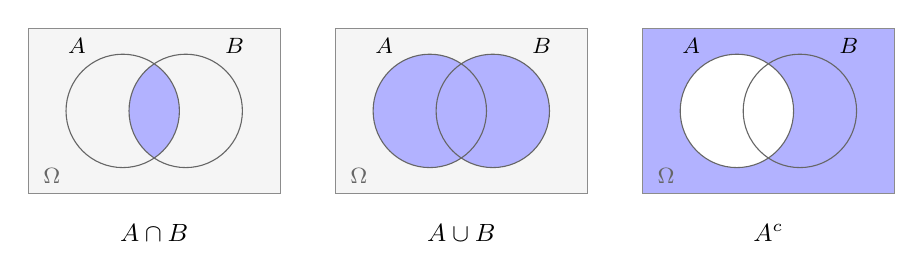
\begin{tikzpicture}[x=1cm,y=1cm,font=\small]
  \draw[black!45,fill=black!4] (0,0) rectangle (3.2,2.1);
  \begin{scope}
    \clip (1.2,1.05) circle (0.72);
    \fill[blue!30] (2.0,1.05) circle (0.72);
  \end{scope}
  \draw[black!60] (1.2,1.05) circle (0.72);
  \draw[black!60] (2.0,1.05) circle (0.72);
  \node[font=\footnotesize] at (0.62,1.88) {\(A\)};
  \node[font=\footnotesize] at (2.62,1.88) {\(B\)};
  \node[font=\footnotesize,black!60] at (0.3,0.22) {\(\Omega\)};
  \node at (1.6,-0.5) {\(A\cap B\)};
  \begin{scope}[shift={(3.9,0)}]
    \draw[black!45,fill=black!4] (0,0) rectangle (3.2,2.1);
    \fill[blue!30] (1.2,1.05) circle (0.72);
    \fill[blue!30] (2.0,1.05) circle (0.72);
    \draw[black!60] (1.2,1.05) circle (0.72);
    \draw[black!60] (2.0,1.05) circle (0.72);
    \node[font=\footnotesize] at (0.62,1.88) {\(A\)};
    \node[font=\footnotesize] at (2.62,1.88) {\(B\)};
    \node[font=\footnotesize,black!60] at (0.3,0.22) {\(\Omega\)};
    \node at (1.6,-0.5) {\(A\cup B\)};
  \end{scope}
  \begin{scope}[shift={(7.8,0)}]
    \fill[blue!30] (0,0) rectangle (3.2,2.1);
    \fill[white] (1.2,1.05) circle (0.72);
    \draw[black!45] (0,0) rectangle (3.2,2.1);
    \draw[black!60] (1.2,1.05) circle (0.72);
    \draw[black!60] (2.0,1.05) circle (0.72);
    \node[font=\footnotesize] at (0.62,1.88) {\(A\)};
    \node[font=\footnotesize] at (2.62,1.88) {\(B\)};
    \node[font=\footnotesize,black!60] at (0.3,0.22) {\(\Omega\)};
    \node at (1.6,-0.5) {\(A^{c}\)};
  \end{scope}
\end{tikzpicture}

\emph{方框是 \(\Omega\)，事件是方框里的一块。``且''对应交，``或''对应并，``非''对应取补——中文里含混的连接词，在集合语言里没有第二种读法。}
\end{center}

互斥容易和独立混作一谈，其实两者管的是不同的事。互斥说的是两个事件不共用任何样本点，是集合层面的判断，跟概率怎么分配无关；独立说的是知道一个发生并不改变另一个的概率，要等概率装上去才能谈。两个概率非零的互斥事件一定不独立——一个发生了，另一个就绝无可能，这是能想到的最强依赖。这条对比会在\hyperref[ch:038]{``条件概率、Bayes 与独立性：新信息怎样改变判断''}里兑现。

\subsection{不是每个子集都有资格当事件}

有限的 \(\Omega\) 上，把全部子集都算作事件毫无障碍。连续情形会碰壁：想在 \([0,1]\) 上给每一个子集都配一个与长度相容的数，数学上办不到。所以模型里要单独列出一族被承认的事件 \(\mathcal F\)，它对取补、对可数并封闭，这样``非 \(A\)''与``\(A\) 或 \(B\)''也还留在族里，不至于问着问着问出界。

\(\mathcal F\) 有一个不太数学的读法：它写下了在你这个模型里，哪些问题有概率可言。日志只记了下单与否，``用户当时停在第几屏''就不在 \(\mathcal F\) 里；不是那件事没有概率，是这个模型没给它留接口。为什么某些子集必须排除、排除之后剩下的族长什么样，属于测度论的工作，可参考\hyperref[sec:12-Real-Analysis-Support/05-Measure-Integration-and-Conditional-Expectation/01]{``\(\sigma\)-代数把可观察事件组织成封闭系统''}。眼下只要记住建模三件套里有它一个位置：\(\Omega\) 说清有哪些结果，\(\mathcal F\) 说清哪些集合算事件，剩下的 \(P\) 才是数。

顺带一提离散与连续的区别。可列举的 \(\Omega\)（骰子点数、等待次数）上一切都直白；连续的 \(\Omega\)（灯泡寿命 \([0,\infty)\)、平面落点 \(\Omega\subseteq\R^2\)）会出现一个初看别扭的现象：每个精确点的概率是零，整个区间的概率却是 \(1\)。下一节给出公理后就能看清它为什么不矛盾。

\subsection{同一句话，两个人两个 \texorpdfstring{\(\Omega\)}{Omega}}

来看一个只用中学算术、却让无数人吵翻的问题：一个家庭有两个孩子，已知其中有一个是女孩，两个都是女孩的概率是多少？

假设生男生女各半且互不影响，区分长幼，得到 \(\Omega=\set{BB,BG,GB,GG}\)，四点等可能。``有一个女孩''对应 \(\set{BG,GB,GG}\)，把观察范围收进这三点，只有 \(GG\) 全是女孩，答案 \(1/3\)。

但那句``已知''是怎么来的？如果消息来自``我在小区里碰到了这家的一个孩子，是个女孩''，试验就不止生育这一层，还多了``碰到的是哪一个''。此时一条完整记录是家庭构成与被碰到的孩子的配对，共八个等可能样本点；碰到女孩的有四个，其中来自全女孩家庭的占两个，答案是 \(1/2\)。

\begin{center}
\begin{tikzpicture}[x=1cm,y=1cm,font=\footnotesize]
  \fill[blue!12] (0,0) rectangle (2.2,0.9);
  \fill[blue!12] (1.1,0.9) rectangle (2.2,1.8);
  \fill[blue!30] (1.1,0) rectangle (2.2,0.9);
  \draw[black!55] (0,0) rectangle (2.2,1.8);
  \draw[black!55] (1.1,0) -- (1.1,1.8);
  \draw[black!55] (0,0.9) -- (2.2,0.9);
  \node at (0.55,1.35) {\(BB\)};
  \node at (1.65,1.35) {\(BG\)};
  \node at (0.55,0.45) {\(GB\)};
  \node at (1.65,0.45) {\(GG\)};
  \node[black!75] at (1.1,2.15) {模型甲：只记家庭构成};
  \node[black!75] at (1.1,-0.5) {四点等可能，答案 \(1/3\)};

  \begin{scope}[shift={(4.6,0)}]
    \fill[blue!12] (1.0,0) rectangle (2.0,0.9);
    \fill[blue!12] (2.0,0.9) rectangle (3.0,1.8);
    \fill[blue!30] (3.0,0) rectangle (4.0,1.8);
    \draw[black!55] (0,0) rectangle (4.0,1.8);
    \foreach \x in {1.0,2.0,3.0}{\draw[black!55] (\x,0) -- (\x,1.8);}
    \draw[black!55] (0,0.9) -- (4.0,0.9);
    \node at (0.5,1.35) {男}; \node at (0.5,0.45) {男};
    \node at (1.5,1.35) {男}; \node at (1.5,0.45) {女};
    \node at (2.5,1.35) {女}; \node at (2.5,0.45) {男};
    \node at (3.5,1.35) {女}; \node at (3.5,0.45) {女};
    \node[black!70] at (0.5,2.0) {\(BB\)};
    \node[black!70] at (1.5,2.0) {\(BG\)};
    \node[black!70] at (2.5,2.0) {\(GB\)};
    \node[black!70] at (3.5,2.0) {\(GG\)};
    \node[black!75] at (2.0,2.5) {模型乙：再记``碰到的是哪个孩子''};
    \node[black!75] at (2.0,-0.5) {碰到女孩的四格里两格来自 \(GG\)，答案 \(1/2\)};
  \end{scope}
\end{tikzpicture}

\emph{浅色格是与``看到一个女孩''相容的结果，深色格是全女孩家庭。同一句中文，两种试验，两个 \(\Omega\)，两个答案。争论双方谁都没算错，他们只是在两张不同的图上数格子。}
\end{center}

三门问题、检验悖论、幸存者偏差都是这个形状：主持人按什么规则开门、你是在哪个时刻走进车站、返航的飞机为什么是你唯一能看到的样本——把这些写进 \(\Omega\)，争论就散了；不写进去，双方各自的算术都无懈可击，结论却对不上。碰到概率争论时，先别急着检查算式，先请两边各自把一条完整记录写出来。

至此三件套只装好了前两件：结果有哪些，哪些集合算事件。下一节给这些事件指派数，并追问这种指派最少要守住哪几条规矩才不会自相矛盾。
